\documentclass[letter,12pt]{article}
\usepackage[pdftex]{graphicx} % Embedding graphics
\usepackage{grffile} % Embedding graphics with spaces
\usepackage{color} % Using colour
\usepackage[margin=1in,top=1in]{geometry} % Set margins
\usepackage{parskip} % No idea
\usepackage{setspace} % No idea
\usepackage{fancyhdr} % Better headers
\usepackage{indentfirst} % Indent first paragraph
\usepackage{placeins} % To force images to not behave stupid as hell
\usepackage{amsmath} % Fancy math functions
\usepackage{amsfonts}
\usepackage{pdfpages}
\usepackage{hanging} % hanging indent
\usepackage{enumitem}
\usepackage{units}
\usepackage{longtable}
\usepackage[hang,flushmargin]{footmisc} 
\usepackage{pdflscape}
\usepackage{geometry}
\usepackage{hvfloat}

% Header Setup
\pagestyle{fancy} 
\fancyhf{}
\rhead{Aaron Rudkin}
\lhead{\textbf{Electoral Returns to Cabinet Membership: Canada}}
\fancyfoot[C]{\thepage}
\renewcommand{\headrulewidth}{1.2pt}
%*************

% Footer for landscape page.
\fancypagestyle{fancynohead}{
\fancyhf{}
\fancyfoot[C]{\thepage}
\renewcommand{\headrulewidth}{0pt}
}
% *******

% Setup for title page
\newcommand*{\customTitle}{\begingroup
\pagestyle{empty}
\vspace*{0.05\textheight}
\noindent\Huge\bfseries Electoral Returns to Cabinet \\ Membership: Canada
\vspace*{0.05\textheight}

\noindent\Large \textsc{Aaron Rudkin\footnote{My thanks to Michael F. Thies, Miriam Golden, Jeff Lewis, and James Tong, for input at various stages during this project, and to Michael Mulley of OpenParliament.ca for facilitating data collection on legislator speeches. Any errors or omissions are my own. A note on language: the convention within Canada is to refer to ``cabinet'', without the use of articles and lowercased, rather than ``the Cabinet''. Replication data and code is available at: \textcolor{blue}{https://github.com/aaronrudkin/CabinetEffect}.}}
\vspace*{0.1\textheight}

\normalsize
\textbf{\underline{Abstract}}

\textmd{Past research offers competing theories about the electoral value of cabinet membership. Some authors identify the electoral benefit of developing a ``personal vote'', while others demonstrate a party-level ``cost of governing'' stemming from broken or under-realized policy promises, attribution of blame to governing parties, and the accumulation of grievances. Adjudicating this question is complicated by sample selection biases with respect to incumbents who choose to run for re-election and endogeneity with respect to those offered cabinet positions. I examine Canadian data post-1945 and find a modest but substantively relevant benefit of 1-3\% vote share across model specifications. Subsequently, I conduct a mediation analysis and identify increased media coverage as a plausible explanation of the electoral return to cabinet. Understanding cabinet membership as producing an electoral return adds to our understanding of individual incentives to join cabinet and party-level strategic considerations when forming cabinet.}

\newpage
\endgroup}
%*************

\begin{document}
\customTitle

\setlength{\parindent}{24pt}
\setstretch{2}
\pagenumbering{arabic}

\subsection*{Introduction}
In studies of parliamentary systems, cabinet formation has primarily been considered from the strategic perspective of parties and coalitions. But parties are not monoliths, they are comprised of individuals with individual preferences and goals (M{\"u}ller and Str{\o}m 2000). It is individuals who must decide whether or not to lobby for a cabinet position, and if extended an invitation whether or not to accept it. What are the costs and benefits to a member of parliament of joining the cabinet? \textit{Specifically, do cabinet ministers receive an electoral return in exchange for joining cabinet?} Prior theories of legislator behaviour are unclear as to whether cabinet membership ought help or hurt re-election efforts. I show that in the Canadian case, cabinet ministers receive a small but substantively meaningful advantage of 1-3\% vote share, durable across model specifications and approaches, and that increased media exposure is a plausible mechanism that translates cabinet membership to improved electoral performance.

Two theories in the literature offer competing predictions about the direction of this effect. (1) At the party level of analysis, governments have been shown to pay a ``cost of governing'': an expectation that once elected to government, they will face electoral punishment in subsequent elections.\footnote{Subsequent work has considered the ``cost of governing'' as a reversion to the mean: that the departure from the ordinary is a party being swept into government, not the apparent ``punishment'' once elected. Even if this is so, perhaps some members of a party are more able than others to translate the unexpected success of the wave they rode into government on into durable electoral gains, and so the overall question remains.} Does this phenomenon translate to individual level performance? If the electorate punishes a governing party, aren't cabinet ministers most vulnerable as the public face of the party's policies? (2) Incumbents benefit from cultivating a ``personal vote'', separate from their party, which they do in part through position taking and credit claiming. In parliamentary countries, where governments maintain tight control of the legislative agenda and voting, cabinet ministers are uniquely well-suited to cultivate a personal vote. 

A functionalist explanation would argue that legislators must believe cabinet membership offers an electoral advantage, or else they would not participate in cabinet, but legislators are not single-minded seekers of re-election. They also desire the ability to achieve policy outcomes, personal and career satisfaction, service to their party, and financial reward (Fenno 1978). The interplay between these factors reinforces the need to assess each. Correctly understanding the risks and payoffs of joining cabinet is relevant to the decision calculus of individual MPs as well as party electoral strategy. Considering cabinet membership as a ``special type'' of incumbency, this analysis also speaks to studies of incumbent electoral advantage more broadly.

Answering this question is methodologically fraught. Parties have access to private signals and data about legislator performance that are opaque and inaccessible to the outside world. Selection into cabinet is not exogenous to electoral performance, both because of reverse causality--more popular candidates are selected into cabinet--and because of omitted common causes of popularity and cabinet selection. Moreover, incumbents choose to retire or run for re-election, and this choice itself is endogenous to cabinet membership and to electoral performance.

In the sections that follow, I review past work, describe the original dataset used in the paper, discuss research design and assess the methodological challenges of answering this question. Next, I present empirical results from cross-sectional descriptive and causal models. I review potential mediators as direct tests of theoretical mechanisms. Finally, I conclude with proposals for future extensions of the research agenda.

\subsection*{Two competing perspectives: costs of government and benefits of a personal vote}

Most political scientists assume that politicians and parties are motivated by desire for re-election (Downs 1957; Mayhew 1974). Whatever other goals they wish to achieve -- prestige, policy influence, wealth, power -- they must first secure and retain their electoral mandates. Mayhew offers three mechanisms through which legislators secure re-election: advertising, credit claiming, and position taking. Subsequent work takes a broader view of legislator behaviour and assesses how legislators form relationships with their constituents in order to secure re-election (Fenno 1978).

An essential tension exists in the literature: on one hand, incumbent governments pay an electoral cost for governing (Mershon 1996). This cost is understood as a tendency for governing parties to lose seats when up for re-election. In theoretical terms, opposition parties benefit from being able to make promises without any chance to deliver on them or be held accountable for failing to do so, while government parties are punished for failing to fulfill the promises they made on the campaign trail (Rose and Mackie 1983; Str{\o}m 1990; Narud and Valen 2008; Akkerman and Lange 2012). Likewise, parties in government are penalized for external conditions over which they have little or no control (Achen and Bartels 2016). Strategic models of voting have further argued that voters who prefer policy outcomes between those offered by parties which might plausibly form government are incentivized to always vote out incumbents in order to drag policy to the center over time (Alesina and Rosenthal 1989; Paldam and Skott 1995; Stevenson 2002). But these conclusions speak to the effects of governing on parties, not on individuals within those parties. Cabinet ministers represent the face and voice of government policy making: they design legislation in cabinet meetings, they table legislation in parliaments, they defend legislation in the media, and so it would stand to reason that they are the primary targets of anti-government ire.\footnote{Or indeed, the beneficiaries of pro-governing gratitude in times of strong economic performance--although governing parties lose seats on average, this is not always the case (Powell and Whitten 1993; Fiorina 1981).}

On the other hand, a widely documented incumbent advantage exists in many countries. Incumbents deter credible challengers from within their own party, as well as from competing parties, from standing for election and enjoy resource advantages compared to those competitors that do enter (Erikson 1971; Carson 2005; Ban, Llaudet, and Snyder 2016; Gelman and King 1990). Legislators seek to maximize their electoral advantage while isolating themselves from the electoral costs of governing. Work studying America has observed that particularistic spending and the visibility associated with committee membership are two of the mechanisms by which legislators can grow their ``personal vote''. The personal vote argument is a quandary for legislators: they need support from their party to be nominated, campaign, raise money, and get elected, but otherwise they want to stand out from their party and grow their personal vote. (Cain, Ferejohn, and Fiorina 1987) How can they strike a balance?

The tension here is not mere coincidence: one of the reasons why parties in government fail to deliver on promises is because individual politicians are incentivized to defect from the party line to pursue their own ends. Viewed through the lens of parties as principals and legislators as agents, this incentive compatibility problem explains a great deal about government performance and speaks to why there is a cost of governing at all. Klasnja and Titiunik find that in a variety of Central and South American cases, there is a direct link between weak constraints on personal vote seeking and high costs of governing (Klasnja and Titiunik, 2017).

\subsection*{Cabinet ministers are uniquely situated to develop a personal vote}

In light of this, which countries are most likely to show an electoral return to cabinet membership? The incentives to earn a personal vote vary by electoral and institutional context. Electoral systems, including single-member plurality, where voters choose candidates directly offer the highest incentive to cultivate a personal vote, because individual members can be rewarded at the ballot box by voters (Carey and Shugart 1995).

Incentives matter little if incumbents cannot take advantage of them. The tools available to members seeking a personal vote also vary by context. In America, legislators enjoy more leeway to cultivate a personal vote through position-taking because members are relatively unconstrained in their roll-call voting behaviour.  By contrast, parliamentary systems require majority support of bills to avoid government collapse and early election calls, so they often impose whipped voting, leaving a legislator few opportunities to establish positions distinct from that of their party. Whipped voting is then enforced through institutional arrangements whereby party officials control renomination, so deviation may carry a high price for re-election. Moreover, in parliamentary systems it is typical that cabinet and party leadership of the governing coalition are the originators of most legislation, and legislative majorities protect bills from opposition or backbencher amendments, preventing backbenchers from directly shaping policy or claiming credit for doing so on the campaign trail. Thus, in many parliamentary countries, although the electoral system offers a strong incentive to pursue a personal vote, legislative institutions curb the ability to do so.

Beyond voting and legislating, how else do legislators earn a personal vote? Much of the research on the United States documents individual legislators making use of earmark processes to secure particularistic spending (or even patronage) for their district. But in the parliamentary context, legislators are often unable to do this for the same reason that they cannot directly pass bills. An exception to this rule are cabinet ministers, who exercise control over spending and policy goods within their domain (even if their autonomy is circumscribed by the Prime Ministers who appoint them). Past work  has established that ministers exert considerable control over their policy domain through their power to shape cabinet conversations and set the cabinet agenda (Laver and Shepsle 1996). Expanding on this, Martin (2016) proposes ``executive particularism,'' a mechanism by which cabinet ministers evade restrictions on legislative particularistic spending through their control over the shape of overall party policy and spending within their particular ministry. Those in the cabinet form a sort of cartel where the bulk of the benefits from legislating are targeted to districts represented by cabinet members, less to districts represented by other government representatives, and nearly none to opposition districts. Preliminary work empirically validates this claim: in a variety of national settings finds, districts represented by ministers see greater levels of spending and investment than backbencher districts (John, Ward, and Dowding 2004; Denemark 2000).

In addition to executive particularism, evidence indicates that credit claiming is an important part of the ability to capitalize electorally on the delivery of spending or policy goods (Grimmer, Messing, and Westwood 2012; Bickers, Evans, Stein, and Wrinkle 2007). Because voters lack the resources to correctly allocate credit or blame for a given action, the key to the credit-claiming story is not the ablity to deliver spending or resource commitments, or the magnitude of resources delivered, but rather the ability of the legislator to capitalize publicly.

The means by which members claim credit differ. Grimmer et al. focus on the use of franked (free) mail in the U.S. Congress. Schaffner (2006) finds a positive effect of local news coverage; Boas and Hidalgo (2011) study candidates with community radio licenses in Brazil. A veritable cottage industry has capitalized on internet and social media data to examine the effect of social media's use on re-election (Adler et al. 1998; Spierings and Jacobs 2014; Broockman and Green 2014). Media exposure and events surrounding legislation may also be a driver of electoral success. In a parliamentary setting, ministers are empowered to claim credit. Every ribbon cutting, every project announcement, every factory tour empowers a minister to attract media attention and establish a reputation for delivery.

Beyond news coverage by third party outlets, MPs generate their own coverage through legal allowances to send free mail to constituents, which vary by jurisdiction. Such mail typically contains a mix of politically neutral personal vote cultivation, including photos of the member at events around the district, position-taking, and credit-claiming statements. Although mail privileges are extended to all legislators equally, not all legislators enjoy an equal ability to produce the kinds of inputs that go into mailers. Concrete legislative achievements, speeches in committees, questions asked and answered during question periods, and within-district events like building openings or project announcements all form part of the credit-claiming done through mail. ``Franked'' mail has been considered from an electoral perspective (Cover 1980; Grimmer, Messing, and Westwood 2012). To the extent that ministers enjoy a greater ability to produce these inputs, and thus claim credit, we would expect them to reap electoral rewards.

Martin's ``Policy, Office, and Votes: The Electoral Value of Ministerial Office'' directly tackles the question of measuring the electoral benefit of cabinet. His cross-sectional, descriptive analysis of Irish data post-1980 finds that controlling for other factors, cabinet ministers earn an average of 8.5\% more of their electoral quota (a measure of the number of votes required to be elected\footnote{Ireland uses an STV (single transferable vote) electoral system where voters rank candidates. Each district has several elected members. The electoral quota is a measure of how many ballots must rank a candidate first for the candidate to be elected. As in other STV electoral systems, the weakest overall candidates are dropped and their first-choice votes re-allocated to their voters' second choices until enough candidates meet the quota to fill the all seats in the district.}) from first-choice ballots than non-cabinet ministers, and that this cabinet advantage is sufficient to overcome the ``cost of governing'. Although he does not directly test mechanisms, he theorizes that this is attributable to executive particularism.

\subsection*{Other returns to cabinet membership}
As noted above, direct electoral return is not the only motivation to join cabinet. Cabinet membership has also been studied in terms of personal financial return (Fisman, Schulz, and Vig 2014) and career advancement (Squire 1988). The theory here is not that the offer of cabinet membership or the decision to accept an offer is exclusively driven by electoral calculus, but rather that in addition to these already documented advantages, the perception of electoral benefit can affect legislator decision-making. In some countries, the personal vote is not the only channel through which cabinet ministers receive electoral reward. In countries where renomination is contentious, competitive, and party-controlled, party elites including cabinet ministers can receive a bonus toward renomination (Golden and Picci 2015). In countries with closed-list proportional representation, parties can directly protect cabinet ministers from electoral threat by moving valued incumbents so high on the electoral list that they are guaranteed re-election.

\subsection*{The Canadian case}
I introduce Canada as a case through which to answer the question about whether cabinet ministers gain or lose electorally from their positions in government. Canada represents a useful case to study when looking for an electoral return to cabinet due to institutional and cultural features and the presence of data necessary to directly test proposed mechanisms. 

Canada is a parliamentary democracy whose lower house is elected by a single-member plurality electoral system. The single-member plurality system ensures a strong incentive to seek a personal vote (Carey and Shugart 1995). Two parties have alternated in government since 1867: the Liberal Party and the Progressive Conservative Party (after 2004, renamed the Conservative Party). Minor parties, including both those organized around regional concerns and those organized around national concerns, have achieved some electoral success and periodically been the largest opposition party. The effective number of parties\footnote{A measure of party competition developed by Laakso and Taagepara (1979), where $N = \frac{1}{\sum_{i=1}^n p_i^2}$, with parties 1 through \textit{n} occupying a $p_i$ share of seats.} during the time studied varies from 1.5 to 3.2 (i.e. in general more political parties than the United States, but many fewer than true multi-party competitive systems such as the Netherlands). This makes Canada a good milieu to assess returns to cabinet because a competitive electoral environment makes it more likely that electoral rewards and punishment take place at the ballot box, rather than primarily through the private workings of a single dominant party. Moreover, the knowledge that incumbent parties and legislators can face a credible electoral threat ensures that electoral strategy is a relevant part of their decision calculus.

Canadian governments are single-party governments, and governments without majority support typically eschew formal agreements with other parties.\footnote{Since the establishment of parliamentary democracy in 1867, no coalition governments have occurred. Opposition parties have proposed toppling minority governments by forming a coalition on several occasions, but never followed through.} In countries with coalition governments, personal benefits (or costs) to joining cabinet compete with complicated party-level strategic considerations: for example, it is widely considered that the U.K. Liberal Democratic Party's decision to form a coalition government with the Conservative Party cost them substantial electoral support in the subsequent parliamentary election. In the absence of coalitions, the relationship between costs of governing and individual personal vote incentives is clearer.

Candidates typically run in districts near where they reside, although the parachuting (carpet-bagging) of star candidates into politically opportune districts does occur (Koop and Bittner 2011). Incumbents do not switch districts in subsequent elections (except as a consequence of periodic and non-partisan redistricting). In countries such as the United Kingdom where district switching is known to occur, measuring incumbency advantage is more difficult due to endogeneity caused by candidates favoured by their parties being shuttled into safer seats; direct comparisons across elections are impossible.

Elections in Canada are relatively low cost, with bans on corporate and union donations. Most elections in recent years have had a substantial public funding component. In other countries where fundraising is a substantial part of the electoral process, cabinet ministers may attract additional financial support from parties, interest groups, and constituents alike, but in Canada we can rule out fundraising and financial involvement of interest groups as drivers of incumbent re-election performance, as well as ensuring that beyond denial of renomination, parties have relatively little financial influence over incumbent re-election.

Canadian prime ministers enjoy latitude to make cabinet appointments as they see fit, subject to no formal constraints on their power. There are, however, norms that serve as \textit{in}formal constraints. These include ensuring the representation of every province in cabinet, the allocation of certain portfolios to relevant geographies (for example, the Fisheries ministry is traditionally given to an MP from one of Canada's coastal provinces), and increasingly a desire to represent diversity of gender and ethnicity. Cabinet ministers are generally expected to be or become bilingual. These constraints are instructive when later considering the selection problems that complicate this paper's analysis. A prior survival analysis of cabinet entry in Canada found that gender, legal experience, education, age, and past ministerial tenure were major predictors of selection into cabinet (Kerby 2009). Cabinets in Canada have become increasingly professionalized and technocratic, a trend also observed in other developed democracies (Lammers and Nyomarkay 1982; Pekkanen, Nyblade, and Krauss 2013; Berlinski, Dewan, Dowding, and Subrahmanyam 2009).

Canadian legislative behaviour is characterized by strict party discipline. Elected representatives are expected to support their party's policy priorities in virtually all cases, and ``conscience votes'' are only allowed when it is believed that the member's defection will not jeopardize the overall outcome of the vote. Expulsion from cabinet, from caucus, or denial of renomination are the primary punishments available to enforce party discipline. Switching between major parties (``crossing the floor'') is rare. Nominations are the prerogative of the local party office, and there are no public primary elections. Party organizations by custom do not remove incumbents for reasons other than scandal or failure to vote with party leadership. 

Legislation in Canada is introduced in the House of Commons by a minister responsible for the portfolio the legislation affects. Backbenchers and opposition members of parliament are permitted to introduce ``private members bills'' through a lottery system, but in practice these are rarely scheduled for further debate or committee referral, have little chance of passing, and are generally symbolic resolutions with no financial outlay or legal-regulatory changes. As noted above, these constraints are precisely why we should expect an advantage to cabinet membership to emerge.

Canada is notable among developed parliamentary democracies for its low incumbent re-election rates, by some measure the lowest of its peers.\footnote{Although some work suggests that an advantage for incumbents nevertheless exists (Kendall and Rekkas 2012).} This is a feature of interest: in a situation where incumbent survival is low, either due to withdrawal (from strategic exit; health; or death), denial of renomination, or loss, newly elected governments (particularly those who have been out of power for some time before winning), are forced to assemble a cabinet from caucuses comprised mostly of new, unexperienced legislators (Kerby 2015). Low incumbent survival ensures that legislators must take seriously the threat of loss, while inexperienced cabinets lend plausibility to the idea that those appointed receive a significant boost in profile and exposure as a result of their appointment.

Having observed these relevant institutional features, I return to the question of interest: do cabinet ministers earn an electoral return (or face an electoral cost) from their appointment to cabinet?

\subsection*{Data}
I study an original dataset consisting of candidate-level returns in every Canadian parliamentary election beginning with the 1945 federal election, including by-elections.\footnote{The data was gathered by scraping Library of Parliament sources and then assembling the data into a panel. Inconsistencies in district and candidate naming across elections required the development of a fuzzy matching algorithm to connect candidates across elections.} This consists of 31,633 observations; because my analysis is limited to differences in the performance of incumbent candidates, I subset to only incumbents, leaving 5,535 observations.

In addition to electoral returns, I gathered several other data sets: first, data on incumbent birthdates and genders. Second, data on the status of all legislation introduced in parliament. Third, transcripts of parliamentary debate which I summarize into a measure of activity within the legislature. Finally, data on the number of times each incumbent was mentioned in major media sources during each parliament.\footnote{A discussion of the sources chosen is found in Appendix 2.} The data on legislation, parliamentary speeches, and media mentions was only available digitally beginning in 1993.

\subsection*{Methodological challenges}
The primary design issues with respect to estimating the electoral returns to cabinet membership are sample selection issues and endogeneity.

First, sample selection. We observe vote share only for those candidates who run. Some incumbents do not run for re-election; this may have several causes. One such circumstance is denial of renomination. Although contested renomination processes are rare in Canada and the national party can compel local party offices to accept candidates, scandal-ridden or misbehaving incumbents are occasionally denied renomination (Koehn 1998). When an incumbent fails to be renominated, their omission from the dataset causes what amounts to a sampling bias. Although renomination is not exactly electoral loss, it presumably correlates with an expectation of poor electoral performance. Beyond renomination failures, incumbents can retire. They may do so for personal reasons (including family or health reasons, running for local political office, moving to the private sector) or because they credibly fear electoral defeat and would prefer the grace of retirement, which the literature discusses as ``strategic exit''.\footnote{Incumbents may also retire due to dissatisfaction with office; past work finds this is quite common among early retirements (Hall and Van Houweling 1995; Kerby and Blidook 2011). Satisfaction is clearly a return from office, but it is outside the scope of this paper.} Strategic exits are well-documented in the literature: work in the US context demonstrates incumbents have an awareness of their future electoral chances and many choose to retire rather than lose, particularly those under the cloud of scandal (Hibbing 1982; Jacobson and Dimock 1994; Groseclose and Krehbiel 1994). It is unclear a priori whether or not exits, strategic and otherwise, are likely to bias estimates of cabinet incumbent advantage up or down. The traditional way to correct for sample selection is through the use of a selection model, as in the popular Heckman correction.

Second, endogeneity due to reverse causality or omitted variables: it may be the case that cabinet ministers enjoy an electoral advantage when running for re-election, or it may be the case that prime ministers select cabinet ministers with respect to their expected electoral outcomes. Alternatively, some unmodeled variable may predict both selection into cabinet and subsequent electoral performance. We can consider this in terms of non-random treatment assignment. Non-random treatment assignment particularly presents difficulties when the kinds of people appointed to cabinet and not appointed to cabinet are extremely different (i.e. there is weak common support on predictor covariates between treatment and control groups). Koop and Bittner (2011) argue that ``star candidates'' are much more likely to be appointed to cabinet in Canada. If assignment to treatment is non-random, then the estimation of the effect of cabinet membership may simply be an artifact of those selected into cabinet.

The ideal solution to tackle this problem would be to compel all incumbents to run for re-election indefinitely, randomly assign incumbents to cabinet without respect to their characteristics, and observe their subsequent electoral performance. Reality is not so kind. When studying empirical election performance, it is impossible to correct through endogeneity through experimental design, thus rendering it necessary to apply corrections at the modeling stage. Several popular quasi-experimental designs, including regression discontinuity, are also not viable to address this problem.\footnote{In brief, regression discontinuity designs require an observable latent ``forcing variable'' through which to distinguish between those ``almost appointed to cabinet'' and those ``barely appointed to cabinet'': here, this is impossible. Other designs like instrumental variables require an exogeneous instrument that affects electoral performance only by means of cabinet appointments. I considered two plausible instrumental variables; size of cabinet (rejected because it is not exogeneous: the prime minister can shrink or grow the cabinet) and number of MPs elected by governing party in an MP's province (rejected because it violates the exclusion restriction insofar as party popularity varies by province).}

In lieu of these, I present a ``selection on observables'' approach. Causal identification requires as-if random assignment into a treatment condition. Suppose that we recognize that cabinet membership is not randomly assigned, but instead is assigned probabilistically based on some characteristics of the candidates that we can measure. This assumption is called conditional ignorability: among members who look similar on the characteristics used in the selection model, cabinet members are chosen as-if randomly. Here I am able to rely on earlier work by Kerby (2009) in identifying the mechanisms of cabinet selection. In order to identify the effect of cabinet membership on electoral fortunes, it is necessary to achieve balanced treatment and control groups. Estimation strategies such as matching and weighting can create control groups that are more directly comparable to treatment groups on the characteristics of interest to satisfy conditional ignorability.\footnote{The assumption that conditional ignorability is \textit{fully} satisfied is heroic; regardless, using matching and weighting as estimation strategies to help sustain a selection on observables estimate of the treatment effect will mitigate biases stemming from non-random assignment and provide a measure of robustness against model misspecification (Ho et al. 2007).} In the absence of cleaner causal identification opportunities, I adopt ``selection on observables'' as a ``next best'' option.

I ask the question ``do cabinet ministers enjoy an electoral advantage compared with backbenchers'' and proceed to estimate the size of this advantage compared to the ``costs of governing''.  I present the following modelling approaches:

\setstretch{1.5}
\begin{enumerate}
	\item \textbf{Descriptive models:} Cross-sectional OLS; OLS controlling for past vote share; OLS with within-member fixed effects; OLS correcting for sample selection via Heckman correction (Dependent variable: Vote share).
	\item \textbf{Causal effects: selection on observables:} Matching (Difference in Means) and Weighting (weighted OLS) estimation strategies
\end{enumerate}
\setstretch{2}

Following the presentation of main models, I examine which mediators might explain the effects shown. In the theory section above, I outlined executive particularism, legislative performance, and media exposure as possible mediators (causal channels through which cabinet membership confers an electoral return). I am able to directly test the latter two: legislative performance and media exposure. I find that media exposure is a likely mediator of the cabinet effect.

\noindent The collected variables are as follows:
\setstretch{1.3}
\begin{itemize}
\item \textbf{VotePct}: A dependent variable measuring vote share in the current election. 
\item \textbf{Elected}: A binary dependent variable, used in models where dependent variable is probability of re-election.
\item \textit{CabinetNow}: A binary variable recording if the candidate was a member of the cabinet during the preceding term. \footnote{Canada offers titular ``minister outside cabinet'' positions. These members are involved in cabinet discussions, but have no portfolios or public duties. Some Prime Ministers also appoint junior ministers, who do not typically attend cabinet meetings. I exclude these as well because the theory above argues that the proposed effect comes from the ability to influence cabinet discussions (in the case of the ``executive particularism'' theory) and claim credit as the public face of a ministry (in the case of the ``credit claiming'' theory). This exclusion also helps stabilize the overall size of cabinets between administrations. I do not code exits or role-switching in the middle of government term: this should cause a conservative bias on the coefficient estimate, because evidence suggests that ministerial exit is predicted by poor performance (Berlinkski, Dewan, and Dowding 2010) or scandal (Dewan and Myatt 2007; Dewan and Dowding 2005).}
\item \textit{TermsServed}: The total unbroken number of terms served by a candidate.\footnote{Some members do exit and re-enter parliament, either due to defeat or pursuit of provincial politics. These instances are fairly rare--in part due to Canada's high early voluntary turnover--but nevertheless present. The decision to code the term number this way requires the assumption that members who leave and re-enter ``lose'' some accumulated mindshare or personal vote, but this modelling assumption is less restrictive and more feasible than one that requires collecting data about how many terms members are absent for and what they were doing while absent.} I treat by-elected members as serving a full term. Tenure is modeled in order to capture the accumulated and accumulating effects of prolonged exposure to the public on developing a personal vote.
\item \textit{Party}: Party label the member stood for election under. I recode minor parties or splinter factions to be independent. Models include party fixed effects use independents as the excluded case, although fixed effect estimates are suppressed in the table below.
\item \textit{PartyInGovt}: A binary variable recording whether the candidate is running for the party currently in power? This variable accounts for the ``electoral costs of governing''.
\item \textit{Province}: Province where the candidate is running for re-election.
\item \textit{Age}: The age of the candidate at the time of the election. Data is only available for a subset of candidates who were elected to office at least once and only used in ancillary models.
\item \textit{Gender}: A binary variable recording candidate gender, where the value ``1'' refers to a female candidate.
\item \textit{PastLawJob}: Canadian incumbents submit an occupational designation when they appear on electoral ballots; I code this variable as 1 if the occupation listed reflects legal experience.\footnote{In specific, any occupation matching the following: lawyer, barrister, notary, barrister-at-law, solicitor, notary public, law professor, barrister \& solicitor, judge, law teacher, barrister-solicitor, law, professor of law, retired judge, lawyer (retired), lecturer in law. I exclude paralegals, legal assistants, and mediators.} This variable has been found to be relevant for selection into cabinet. (Kerby 2009)
\item \textit{NumWordsSpoken}: The number of words spoken by an incumbent candidate in the previous parliamentary session: this is a rough measure of the legislator's activity in parliament, in light of constraints on non-speech legislative activity.\footnote{Parliamentary transcripts do not have sufficiently granular timestamps to assess total speech time. The inclusion of interruptions and exclamations in the parliamentary record renders words a better measure of contribution than number of distinct speeches, although of course some members are more parsimonious than others and so this proxy is a rough operationalization of actual parliamentary behaviour.} When used, this variable is log-transformed because of distributional skew and order-of-magnitude differences in the data.
\item \textit{MediaMentions}: The number of times an incumbent MP was mentioned in major Canadian media sources since the previous election. When used, the variable is log-transformed.
\end{itemize}
\setstretch{2}

\subsection*{Results: OLS}

I begin by presenting a suite of cross-sectional models to determine the association between cabinet membership and electoral outcomes, controlling for other covariates. In order, I present three main specifications; each regresses vote share against cabinet membership, party in government, tenure, and fixed effects. Specification 1 includes party fixed effects; specification 2 includes party fixed effects and controls for the incumbent's previous performance; specification 3 adds within-member fixed effects.\footnote{Alternate specifications including party-year fixed effects and controlling for gender and past legal experience all produce results comparable to Specification 1 and are available in the replication archive for this paper.} Coefficient estimates are all positive, centering between 0.6 and 2.4 points; confidence intervals exclude zero for the first two specifications. Recall that because of the structure of member fixed effects, the final specification is the most conservative. 

To assess what this means in concrete terms, 621 contests in the dataset were decided by margins below 2.4\%, including 34 in the most recent federal election; 162 contests, including 10 in the most recent federal election, were decided by a margin below 0.6\%. Given that a swing of 34 seats would typically be enough to change the party forming government and a swing of 10 seats would typically be enough to move from a minority government to a majority government, I interpret these estimates as substantively modest but relevant. The cost of government similarly varies, but it is consistently negative and moderate. Together, I interpret these results as suggestive that cabinet ministers can partially overcome the cost of governing.\footnote{Logistic regressions that estimate the relationship between cabinet membership and probability of re-election are presented in Appendix 1: cabinet membership is associated with a 5\% higher probability of re-election across specifications.}

\setstretch{1}
\input{"Includes/table1"}
\setstretch{2}
\pagebreak

\subsection*{Results: Heckman Correction}

These results are suggestive, but suffer from at least two forms of selection we will want to correct for. First, sample selection bias induced by early exit (whether strategic or not). I correct for this sample bias using the Heckman correction (Heckman 1979) estimated via full information maximum likelihood. The Heckman correction estimates two models: whether or not a member will run for re-election; and then the model of interest. In order to do this, I add synthetic observations for incumbent members who exit the dataset prior to being defeated. (n=844) These observations contain all of the predictor fields but are missing outcome data because the incumbents did not actually run. The Heckman correction uses these observations in the first stage model, but not the second stage model. My selection model includes cabinet membership, party in government, length of tenure, prior vote performance, gender, province, and past legal experience as predictors. I include provincial label because provincial political opportunities and competition may differ systematically between provinces; gender because women may face differential pressures to exit early; and past legal experience as a weak proxy for external economic opportunities available to the member; and prior vote performance to model strategic exit. The outcome model is estimated as in the first results selection:

\setstretch{1}
\input{"Includes/table2"}
\setstretch{2}

Again, specification 1 provides the base model; specification 2 controls for individual past performance; specification 3 adds member fixed effects (the coefficient now explains within-individual variation in performance rather than between-individual). The Heckman-corrected models produce comparable but not identical results to the original models. Coefficient signs are positive and CIs center between 0.6 and 2.4 points; confidence intervals exclude zero for the first two specifications, but again not for the within-member model. Once again, the failure of the third model to exclude the null hypothesis is likely attributable to the conservative model specification. It seems that early exit, strategic or otherwise, does not substantially impact the model estimates.

\subsection*{Results: Selection on Observables}

The other major threat to estimate validity is endogeneity (reversed causality or effects caused by an omitted variable). As described above, I mitigate this by considering cabinet as a selection on observables process. Under the conditional ignorability assumption, selection on observables produces a causally identified estimate of a treatment effect. I use two strategies to achieve balanced treatment and control samples. First, I use matching. I match on gender, terms served, previous performance, party in government, past legal experience, and province. Matching takes every treated observation (cabinet minister) and attempts to find the closest possible control observation. In other words, it allows us to directly observe the world where those selected into cabinet were similar to those not selected into cabinet. Because I am matching on several covariates, matches may be imperfect (the data set may not contain an incumbent who is identical to a given cabinet minister in all the relevant ways): I compensate for this by employing a bias-corrected matching strategy, which penalizes inexact matches and allows for an accurate estimation of uncertainty (Abadie and Imbens 2011).

\begin{figure}
\centering
\caption{Covariate Balancing (Matching)}
\includegraphics[width=0.45\textwidth]{"Includes/love_plot_match"}
\includegraphics[width=0.45\textwidth]{"Includes/love_plot_match_age"}
\end{figure}

Both matching models produce substantially better balance between treatment and control units than the original dataset. This test produces an effect (mean difference in means between treated and matched controls) of 1.70\% across the entire dataset (confidence interval using Abadie-Imbens standard errors spans 0.20\% to 3.21\%). Matching additionally on age, which requires discarding some observations for which data is missing, generates a confidence interval from 0.93\% to 3.81\%, centered at 2.37\%. Estimate magnitudes are comparable to the initial descriptive models.

Matching is a special case of weighting. Instead of matching each treatment observation to a control observation, weighting manipulates the relative importance of control observations to induce a control population that is as similar as possible to the treated population across the covariates weighted on. Weighting provides a measure of double robustness: whereas a conventional regression model is subject to bias in effect estimates if it is misspecified, under weighting, the selection model and effect estimation model lend each other mutual strength and reduce the dependence of the effect estimates on either model being specified correctly. To be specific, I implement entropy balancing, a modern approach that ensures maximum possible covariate balance (Hainmueller 2012). I implemented a weighted least squares regression using the resulting weights. Entropy balancing has achieved complete balance between treatment and control units.

\begin{figure}
\centering
\caption{Covariate Balancing: Entropy Balancing (Weighting)}
\includegraphics[width=0.55\textwidth]{"Includes/love_plot_weight"}
\end{figure}

The resulting effect is estimated at 1.25\%, with a confidence interval spanning from 0.57\% to 1.93\%. Below I present regression estimates for the resulting weighted least squares regression:

\setstretch{1}
\input{"Includes/table3"}
\setstretch{2}
\pagebreak

\subsection*{Mediation and Direct Tests of Theory}

Although it was impossible to gathering direct district-level expenditure data to test the theory of executive particularism, I have gathered data about other behavioural ways in which Cabinet Ministers are different -- and similar -- to backbench members. These are potential mediators which explain how cabinet membership provides an electoral return. I explore three legislator outputs. 

I begin by examining participation in parliament. I gathered transcript data from every parliamentary debate from 1993 onwards. Parliamentary debate transcripts do not have adequate timing data to verify speaking lengths, applause data, or other measures of legislator efficacy, but it is possible to gather data on speaking. I record the number of words spoken by each representative for each parliament. The median speaker speaks 68,000 words per parliament, with an interquartile range of 31,000 to 123,000 words. Outliers on the low end including members acutely dying of illness, in the process of retiring, and the Speaker of the House (who never speaks in a personal capacity). Outliers on the high end seem to have no consistent pattern. An exploratory regression shows that while cabinet ministers speak slightly more often than backbenchers of the same party, the differences are substantively small. The Canadian parliament adopts an institutional speaking arrangement which Proksch and Slapin (2015) deem to be the most ``open'' speaking time allocation rule among comparative systems, so backbenchers who wish to speak on a bill or resolution can typically do so. Moreover, the average member of the party in government speaks slightly less compared with opposition members. I offer a few preliminary explanations for this: first, because government members can constructively shape legislation in private caucus meetings, while the opposition must do so in parliament. Second, opposition parties have fewer members but must critique the same number of portfolios as the government must defend, and so the average opposition member has more duties inside the legislature. 

Among individual level covariates, gender, length of tenure, age, and past electoral performance were poorly predictive or not at all. Only past experience as a lawyer was strongly associated with parliamentary speech, which may be proxying for self-selection into speech based on a member's confidence in their public speaking ability or higher latent legislator quality. Regardless, because there is no real association between cabinet membership and parliamentary participation, it is unlikely to be a useful mediator.

\begin{figure}
\centering
\caption{Parliamentary Participation}
\includegraphics[width=0.45\textwidth]{"Includes/participation_govopp"}
\includegraphics[width=0.45\textwidth]{"Includes/participation_cabinet"}
\end{figure}

Next, I consider legislative output. This is an inappropriate mediator for precisely the opposite reason: virtually all legislative output in Canada flows through cabinet. Any Canadian parliamentarian can table legislation, but they are not entitled to scheduling a vote or referring the bill to committee. Although several ``private members bills'' (bills not sponsored by a cabinet minister) pass each year, only one fifth of all legislation is passed in this way. Backbenchers do table bills with an expectation that they will not become law -- and this can still be a form of position taking -- but it is difficult for them to translate those bills into output for their constituents. Of 1,647 backbenchers who have served since 1993, only 31 have successfully passed a single bill, and only 4 have passed more than one. Many of those bills are symbolic only and do not involve regulatory changes or financial outlays.

A more troublesome limitation of this data is that while cabinet membership is virtually necessary to pass legislation, it is not sufficient. Most cabinet ministers also never table or pass a bill. Of 188 cabinet ministers in the same period, only 27 have passed bills. This is partially due to the increasing practice of tabling omnibus legislation that covers multiple domains: although the Minister of Northern Affairs might rarely table legislation, omnibus legislation including a section dealing with Northern Affairs is common. This is especially true of the federal budget, which is introduced by the Minister of Finance but affects virtually all portfolios. Thus, while it is likely that credit-claiming about legislation passed is part of the story of electoral returns to cabinet membership, it cannot be directly measured through a count of legislation a minister has tabled or passed.

Finally, I examine media mentions. Cabinet ministers may possess superior credit-claiming abilities through increased media exposure. While government members do earn slightly fewer media mentions than opposition members, cabinet ministers buck this trend, earning far more mentions than government backbenchers. The median MP-parliament observation in the dataset is mentioned 69 times (interquartile range from 27 to 201): over government terms that average below 4 years and a nine month period of parliamentary activity, this amounts to 2 mentions per month. The median cabinet minister-term observation is mentioned 371 times (interquartile range 175 to 664). A cross-sectional regression of media mentions against all individual predictors shows that cabinet membership has the strongest association with increasing media coverage. Prime Ministers, being ``first among equals'' earn substantially more mentions than other cabinet ministers (the median Prime Minister-term observation is mentioned 5,904 times). The coefficient on cabinet membership suggest a closer association than past legal experience, tenure, past vote share, gender, or province of origin.

\begin{figure}
\centering
\caption{Media Mentions}
\includegraphics[width=0.45\textwidth]{"Includes/media_govopp"}
\includegraphics[width=0.45\textwidth]{"Includes/media_cabinet"}
\end{figure}

Although the data on media mentions is limited to post-1993 observations, I perform a mediation analysis to attempt to explain what proportion of the electoral return to cabinet membership can be accounted for by increased media mentions. My mediation model can be best understood through a causal graph:

\begin{figure}
\centering
\caption{Causal Mediation Pathway}
	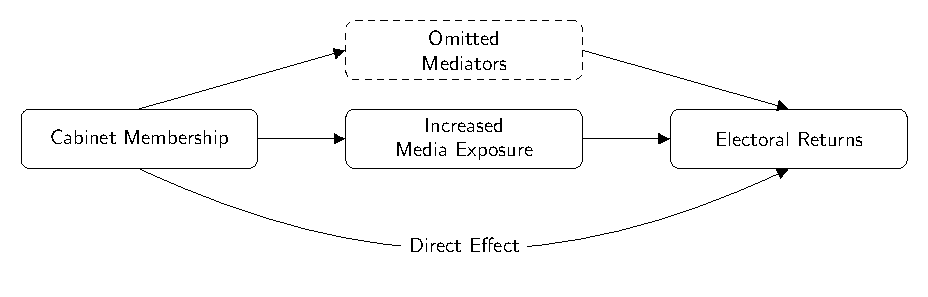
\includegraphics[width = 0.8\textwidth]{Includes/flowchart}
\end{figure}

Mediation analysis separately fits two models: a model predicting the mediator (in this case, media mentions) including the treatment covariate (cabinet membership) and other covariates and a model predicting the outcome including the mediator, the treatment, and other covariates.\footnote{The methodological basis for mediation analysis is explored in Imai, Keele, and Tingly (2010).} These two models form an input to the mediation analysis, which decomposes the effect of the treatment into two components: the proportion of the relationship explained through the mediator, and the proportion which survives the mediation (and is viewed as a ``direct effect'', although the omitted mediators may account for some of the effect). The mediation analysis reveals complete mediation: all of the effect of cabinet membership on vote outcome can be explained by its mediation through media mentions; the remaining direct effect is negative, with a confidence interval admitting zero effect. Total mediation is not surprising: even in a theoretical vacuum, it would not be assumed that cabinet membership \textit{directly} bestows any electoral reward; rather, cabinet membership grants access to resources which in turn lead to electoral reward. \footnote{Although the ordering of the covariates here makes mediation analysis an appropriate tool, a similar result occurs when adding logged media mentions to an OLS regression; the coefficient for cabinet (direct effect) is negative with a confidence interval including zero, while the coefficient for media mentions is high and positive.}

\newpage
% The mediation package doesn't support stargazer, so I put this directly
\setstretch{1}

\begin{table}[!htb] \centering 
  \caption{Mediation Analysis: Effect of Cabinet Membership through Media Mentions} 
  \label{} 
  \begin{tabular}{@{\extracolsep{5pt}}lc} 
\\[-1.8ex]\hline 
\hline \\[-1.8ex] 
& Estimate\\
\cline{2-2} 
\\[-1.8ex]
Mediated Effect & $2.56^{***}$ \\
& (1.82, 3.32) \\
& \\
Direct Effect & $-0.84$ \\
& (-2.73, 1.01) \\
& \\
Total Effect & 1.73 \\
& (-0.21, 3.50) \\
\\[-1.8ex]\hline 
\hline \\[-1.8ex]
\end{tabular}
\end{table}
\setstretch{2}

This mediation analysis suggests that increased media exposure is likely to be a mediation pathway through which cabinet membership translates into electoral reward. Two disclaimers are in order: First, because of limitations of the media mention data, this is underpowered compared to the initial models. Second, mediation analysis relies on on a strong underlying assumption called sequential ignorability which cannot be directly tested for and may be heroic in real-world data. However, I provisionally interpret these results as suggestive of one pathway through which cabinet membership brings electoral returns.

\subsection*{Conclusion}
I conclude by summarizing the models presented in this paper. A consistent pattern emerges across model specifications: cabinet membership is associated with a small electoral advantage of 1-3\%.
\begin{figure}[!htb]
\centering
\caption{Estimate of Coefficients Across Models}
	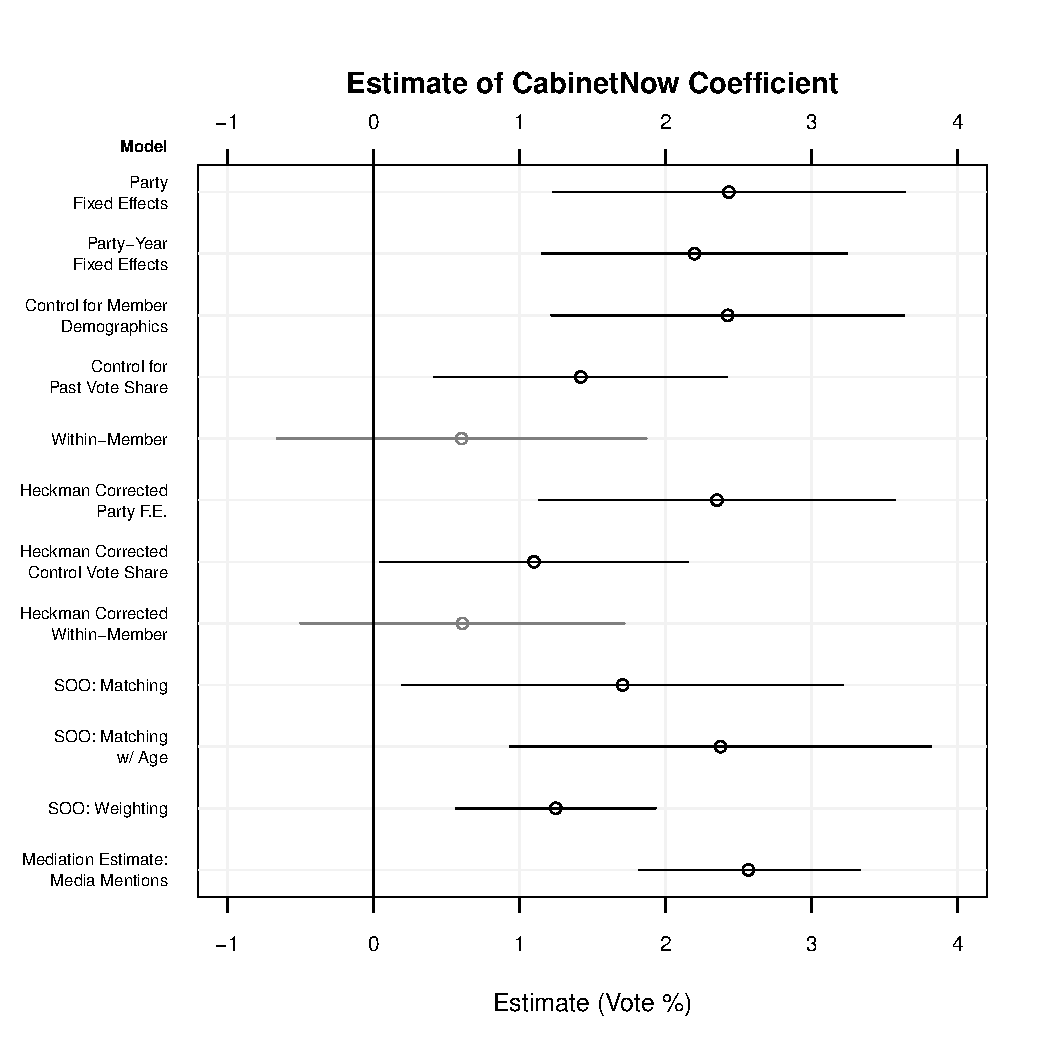
\includegraphics[width = 0.8\textwidth]{includes/estimatePlot}
\end{figure}

Much remains to be done. In future work, additional information on legislative outputs, including direct measurement of MP-district communications, measurements of district-level spending, media mention data for more of the sample, and direct information about re-election campaigns could plausibly bolster or refute the relationship present in this data. In addition, a stronger theoretical basis for the selection model would ensure that conditional ignorability is sustained in the causal models. Modeling MPs who exit (through loss or attrition) and re-enter parliament or collecting data on explicit reasons for attrition may offer insight on the relationship of these processes with personal vote cultivation and electoral returns to cabinet. Finally, it remains to be seen how the result found in Canada translates to other countries: which institutional features are required to observe an electoral return to cabinet, and which other mediation channels can cabinet members use to obtain electoral advantage? 

Re-election motivated incumbents will seek out any opportunity to cultivate a personal vote, especially to inoculate themselves from the costs of governing. In parliamentary systems with strong party discipline, enforced by centralized nomination control, and cabinet domination of the legislative agenda, there are strong incentives but few opportunities for individual legislators to do this. Cabinet ministers, through advantages including particularistic spending and better credit claiming abilities, can plausibly obtain electoral returns from their cabinet position. Across specifications, a modest but substantively relevant association can be observed between cabinet membership and improved electoral returns. An exploration of potential mediators to operationalize credit claiming suggests media coverage is one potential mechanism through which cabinet membership brings electoral returns.

\newpage
\setstretch{2}

\subsection*{Appendix 1: Logistic Regression / Longitudinal Properties}
Incumbents are not solely motivated by \textit{vote} maximization; rather, they are driven by re-election. If the effect of cabinet membership is concentrated among those who already win by large margins, then it is not relevant to the strategic calculus of incumbents or parties. The below logistic regression suggests a 4.8\% average increase in re-election probability for incumbent cabinet ministers (logistic regression fit on true data, predicted probabilities taken by holding all other variables to their true values and varying cabinet membership).

\setstretch{1}
\input{"Includes/appendix_logit"}
\setstretch{2}

In addition, to give a sense of the impact of cabinet membership over a longitudinal time period, I fit a conditional logistic regression model (a logistic regression with fixed effects for each numerical term of service)--this is equivalent to a logistic survival model. The plot below shows the modal Liberal party case. 

\begin{figure}[!htb]
\centering
\caption{Incumbent Longitudinal Survival Rate}
	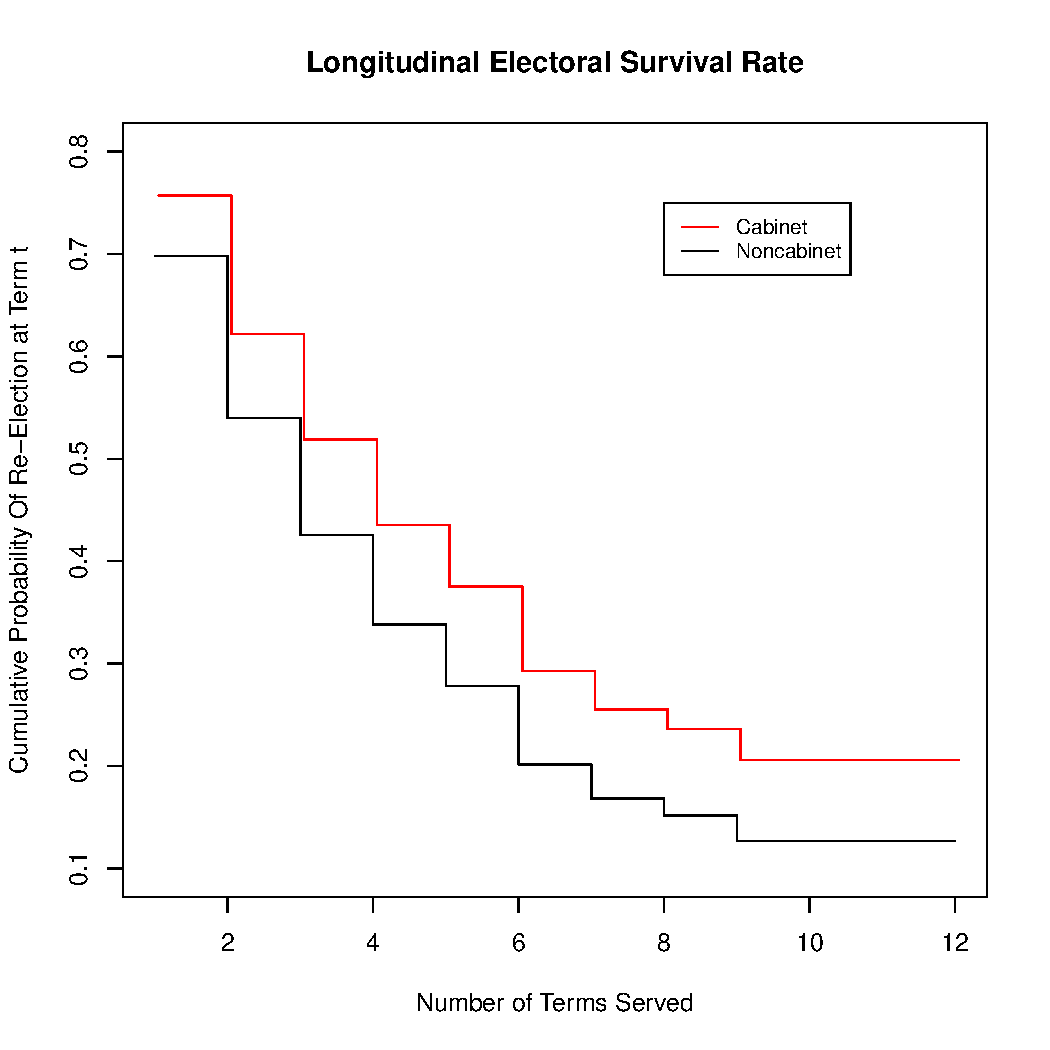
\includegraphics[width = 0.8\textwidth]{includes/cumulative_survival}
\end{figure}
\clearpage
\pagebreak

\subsection*{Appendix 2: Media Sources}
\input{"Includes/appendix_lexisnexis"}

\newpage
\subsection*{References}
\setstretch{1}
\begin{hangparas}{.25in}{1}
Abadie, Alberto and Guido Imbens. ``Bias-Corrected Matching Estimators for Average Treatment Effects.'' \textit{Journal of Business \& Economic Statistics}, 29(1): pp. 1-11. 2011.

Achen, Chris and Larry Bartels. \textit{Democracy for Realists}. Princeton: Princeton University Press. 2016.

Adler, E. Scott, Chariti Gent, and Cary Overmeyer. ``The Home Style Homepage: Legislator Use of the World Wide Web for Constituency Contact.'' \textit{Legislative Studies Quarterly}, 23(4): pp. 585-595. 1998.

Akkerman, Tjitske and Sarah de Lange. ``Radical Right Parties in Office: Incumbency Records and the Electoral Cost of Governing.'' \textit{Government and Opposition}, 47(4): pp. 574-596. 2012.

Alesina, Alberto and Howard Rosenthal. ``Partisan Cycles in Congressional Elections and the Macroeconomy.'' \textit{American Political Science Review}, 83(2): pp. 373-398. 1989.

Ban, Pamela, Elena Llaudet, and James Snyder. ``Challenger Quality and the Incumbency Advantage''. \textit{Legislative Studies Quarterly}, 41(1): pp. 153-179. 2016.

Berlinski, Samuel, Torun Dewan, Keith Dowding, and Gita Subrahmanyan. ``Choosing, moving, and resigning at Westminster, UK'' in Keith Dowding and Patrick Dumont (eds.), \textit{The Selection of Ministers in Europe: Hiring and Firing}. New York: Routledge. 2009.

Bickers, Kenneth, Diana Evans, Robert Stein, and Robert Winkle. ``The Electoral Effect of Credit Claiming for Pork Barrel Projects in Congress''. Presented at Annual Meeting of the American Political Science Association. 2007.

Boas, Taylor and F. Daniel Hidalgo. ``Controlling the Airwaves: Incumbency Advantage and Community Radio in Brazil.'' \textit{American Journal of Political Science}, 55(4): pp. 869-885. 2011.

Broockman, David and Donald Green. ``Do online advertisements increase political candidates' name recognition or favorability? Evidence from randomized field experiments.'' \textit{Political Behavior} 36(2): pp. 263-289. 2013.

Cain, Bruce, John Ferejohn, and Morris Fiorina. ``The Constituency Service Basis of the Personal Vote for U.S. Representatives and British Members of Parliament''. \textit{American Political Science Review}, 78(1): pp. 110-125. 1984.

Cain, Bruce, John Ferejohn, and Morris Fiorina. \textit{The personal vote: Constituency service and electoral independence.} Cambridge: Harvard University Press. 1987.

Carey, John and Matthew Shugart. ``Incentives to Cultivate a Personal Vote: a Rank Ordering of Electoral Formulas''. \textit{Electoral Studies}, 14(4): pp. 417-439. 1995.

Carson, Jamie. ``Strategy, Selection, and Candidate Competition in U.S. House and Senate elections.'' \textit{Journal of Politics}, 67(1): pp. 1-28. 2005.

Cover, Albert. ``Contacting Congressional Constituents: Some Patterns of Perquisite Use.'' \textit{American Journal of Political Science}, 24(1): pp. 125-135. 1980.

Denemark, David. ``Partisan Pork Barrel in Parliamentary Systems: Australian Constituency-Level Grants.'' \textit{Journal of Politics} 62(3): pp. 896-915. 2000.

Downs, Anthony. \textit{An Economic Theory of Democracy}. New York: Harper, 1957.

Erikson, Robert. ``The Advantage of Incumbency in Congressional Elections''. \textit{Polity} 3: pp. 395-405. 1971.

Fenno, Richard F. \textit{Home Style: House Members in Their Districts}. Boston: Little, Brown, 1978.

Fisman, Raymond, Florian Schulz, and Vikrant Vig. ``The Private Returns to Public Office.'' \textit{Journal of Political Economy}, 122(4): pp. 806-862. 2014.

Gelman, Andrew and Gary King. ``Estimating Incumbency Advantage without Bias.'' \textit{American Journal of Political Science}, 34(4): pp. 1142-1164. 1990.

Golden, Miriam and Lucio Picci. ``Incumbency Effects under Proportional Representation: Leaders and Backbenchers in the Postwar Italian Chamber of Deputies.'' \textit{Legislative Studies Quarterly} 40(4): pp. 509-538. 2015.

Grimmer, Justin, Solomon Messing, and Sean Westwood. ``How Words and Money Cultivate a Personal Vote: The Effect of Legislator Credit Claiming on Constituent Credit Allocation.'' \textit{American Political Science Review} 106 (4): pp. 703?719. 2012.

Groseclose, Tim and Keith Krehbiel. ``Golden parachutes, rubber checks, and strategic retirements from the 102nd House''. \textit{American Journal of Political Science}, 38(1): pp. 75-99. 1994.

Hainmueller, Jens. ``Entropy Balancing for Causal Effects: A Multivariate Reweighting Method to Produce Balanced Samples in Observational Studies.'' \textit{Political Analysis}, 20(1): pp. 25-46. 2012.

Hall, Richard and Robert Van Houweling. ``Avarice and ambition in Congress: Representatives' decisions to run or retire from the US House''. \textit{American Political Science Review}, 89(1): pp. 121-136. 1995.

Heckman, James. ``Sample Selection Bias as a Specification Error.'' \textit{Econometrica} 47(1): pp. 153-161. 1979.

Hibbing, John. ``Voluntary Retirement from the U.S. House of Representatives: Who Quits?''. \textit{American Journal of Political Science}, 26(3): pp. 467-484. 1982.

Ho, Daniel, Kosuke Imai, Gary King, and Elizabeth Stuart. ``Matching as Nonparametric Preprocessing for Reducing Model Dependence in Parametric Causal Inference.'' \textit{Political Analysis} 15: pp. 199-236. 2007.

Imai, Kosuke, Luke Keele, and Dustin Tingley. ``A general approach to causal mediation analysis.'' \textit{Psychological Methods}, 15(4): pp. 309-334. 2010.

Jacobson, Gary and Michael Dimock. ``Checking out: The effects of bank overdrafts on the 1992 house elections.'' \textit{American Journal of Political Science}, 38(3): pp. 602-624. 1994.

John, Peter, Hugh Ward, and Keith Dowding. ``The Bidding Game: Competitive Funding Regimes and the Political Targeting of Urban Programme Schemes.'' \textit{British Journal of Political Science}, 34(3): pp. 405-428. 2004.

Kendall, Chad and Marie Rekkas. ``Incumbency Advantage in the Canadian Parliament''. \textit{Canadian Journal of Economics}. 45(4): pp. 1560-1585. 2012.

Kerby, Matthew. ``Worth the wait: determinants of ministerial appointment in Canada, 1935-2008''.
\textit{Canadian Journal of Political Science}, 42(3): pp. 593-611. 2009.

Kerby, Matthew and Kelly Blidook. ``It's Not You, It's Me: Determinants of Voluntary Legislative Turnover in Canada''. \textit{Legislative Studies Quarterly}, 36(4): pp. 621-643. 2011.

Kerby, Matthew. ``Ministerial Careers in Canada'' in Keith Dowding and Patrick Dumont (eds.), \textit{The Selection of Ministers around the World}. New York: Routledge. 2015.

Key, V. O. \textit{Politics, Parties, and Pressure Groups}. New York: Crowell. 1964.

Kla\v{s}nja, Marko and Roc\'{i}o Titiunik. ``The Incumbency Curse: Weak Parties, Term Limits, and Unfulfilled Accountability.'' \textit{American Political Science Review}, 111(1): pp. 129-148. 2017.

Koehn, Miriam. ``Targeted representation? An analysis of the appointment of Liberal candidates in the 1993 and 1997 federal elections.'' \textit{Past Imperfect} 7: pp. 55-86. 1998.

Koop, Royce and Amanda Bittner. ``Parachuted into Parliament: candidate nomination, appointed candidates, and legislative roles in Canada.''. \textit{Journal of Elections, Public Opinion, and Parties}, 21(4): pp. 431-452. 2011.

Laakso, Markku and Rein Taagepera. ``Effective Number of Parties: A Measure with Application to West Europe.'' \textit{Comparative Political Studies} 12(1): pp. 1-27. 1979

Lammers, William and Joseph Nyomarkay. ``The Canadian Cabinet in Comparative Perspective''. \textit{Canadian Journal of Political Science}, 15(1): pp. 29-46. 1982.

Laver, Michael and Kenneth Shepsle. \textit{Cabinet Ministers and Parliamentary Governments}. Cambridge: Cambridge University Press. 1994.

Laver, Michael and Kenneth Shepsle. \textit{Making and Breaking Governments}. Cambridge: Cambridge University Press. 1996.

Martin, Shane. ``Policy, Office and Votes: The Electoral Value of Ministerial Office''. \textit{British Journal of Political Science}, 46(2): pp. 281-296. 2016.

Matland, Richard and Donley Studlar. ``Determinants of Legislative Turnover: A Cross-National Analysis''. \textit{British Journal of Political Science}, 34(1): pp. 87-108. 2004.

Mayhew, David. \textit{Congress: The Electoral Connection}. New Haven: Yale University Press. 1974.

Mershon, Carol. ``The costs of coalition: Coalition theories and Italian governments''. \textit{American Political Science Review}, 90(3): pp. 534-554. 1996.

M{\"u}ller, Wolfgang and Kaare Str{\o}m. \textit{Coalition Governments in Western Europe}. Oxford: Oxford University Press. 2000.

Narud, Hanne and Henry Valen. ``Coalition Membership and Electoral Performance.'' in Str{\o}m, Kaare, Wolfgang M{\"u}ller, and Torbjorn Bergman (eds.), \textit{Cabinets and Coalition Bargaining: The Democratic Life Cycle in Western Europe}. Oxford: Oxford University Press. 2008.

Paldam, Martin and Peter Skott. ``A rational-voter explanation of the cost of ruling.'' \textit{Public Choice}, 83(1): pp. 159-172. 1995.

Pekkanen, Robert, Benjamin Nyblade, and Ellis Krauss. ``The logic of ministerial selection: Electoral system and cabinet appointments in Japan.'' \textit{Social Science Japan Journal} JYT28. 2013.

Proksch, Sven-Oliver and Nathan Slapin. \textit{The Politics of Parliamentary Debate: Parties, Rebels, and Representation.} Cambridge: Cambridge University Press. 2015.

Rose, Richard and Thomas Mackie. ``Incumbency in government: Liability or asset?'' in Daalder, Hans and Peter Mair eds. \textit{Western European Party Systems}. Beverly Hills: Sage. 1983.

Schaffner, Brian. ``Local News Coverage and the Incumbency Advantage in the U.S. House.'' \textit{Legislative Studies Quarterly}, 31(4): pp. 491-511. 2006.

Spierings, Niels and Kristof Jacobs. ``Getting Personal? The Impact of Social Media on Preferential Voting.'' \textit{Political Behavior}, 36(1): pp. 215-234. 2014.

Squire, Peverill. ``Career Opportunities and Membership Stability in Legislatures.'' \textit{Legislative Studies Quarterly}, 13(1): pp. 65-82. 1988.

Stevenson, Randolph. ``The Cost of Ruling, Cabinet Duration, and the `Median-Gap' Model.'' \textit{Public Choice}, 113(1): pp. 157-178. 2002.

Str{\o}m, Kaare. ``A behavioral theory of competitive political parties''. \textit{American Journal of Political Science}, 34(2): pp. 565-598. 1990.
\end{hangparas}
\end{document}